\section{Filtrado de señales}
	\subsection{}
		Acerca del filtro se tiene la siguiente información:
		\begin{enumerate}
			\item Es un filtro pasa-alto y tiene un polo en cero
			\item El polo está ubicado a una distancia $r = 0.9$ del origen en el plano-z
			\item Las señales constantes no pasan por el sistema
		\end{enumerate}
		
		A partir de los datos, se puede deducir que se tiene un rechazo para DC, por lo que la ubicación del cero en el plano complejo debe cumplir:
		\begin{equation*}
			z - 1 = 0 \Longleftrightarrow z = 1
		\end{equation*}
		
		Sabiendo que $z = e^{j\omega}$, al evaluar en $\omega = 0$ se tendrá rechazo de la banda DC. Para la ubicación del polo, se sabe conviene que este esté lo más apegado al cero, de esta forma se tendrá un filtro con mayor selectividad, se comportara como un filtro \textit{notch} 	para DC. Por lo que podemos definir la ubicación del polo en $z_{p} = 0.9$. De esta forma la función de transferencia queda de la siguiente forma:
		\begin{equation}
		H(z) = \frac{z-1}{z-0.9}
		\label{eq:1_filter_transfer_function}
		\end{equation}
		
		Realizando el diagrama de polos y ceros:
		\begin{figure}[H]
			\center
			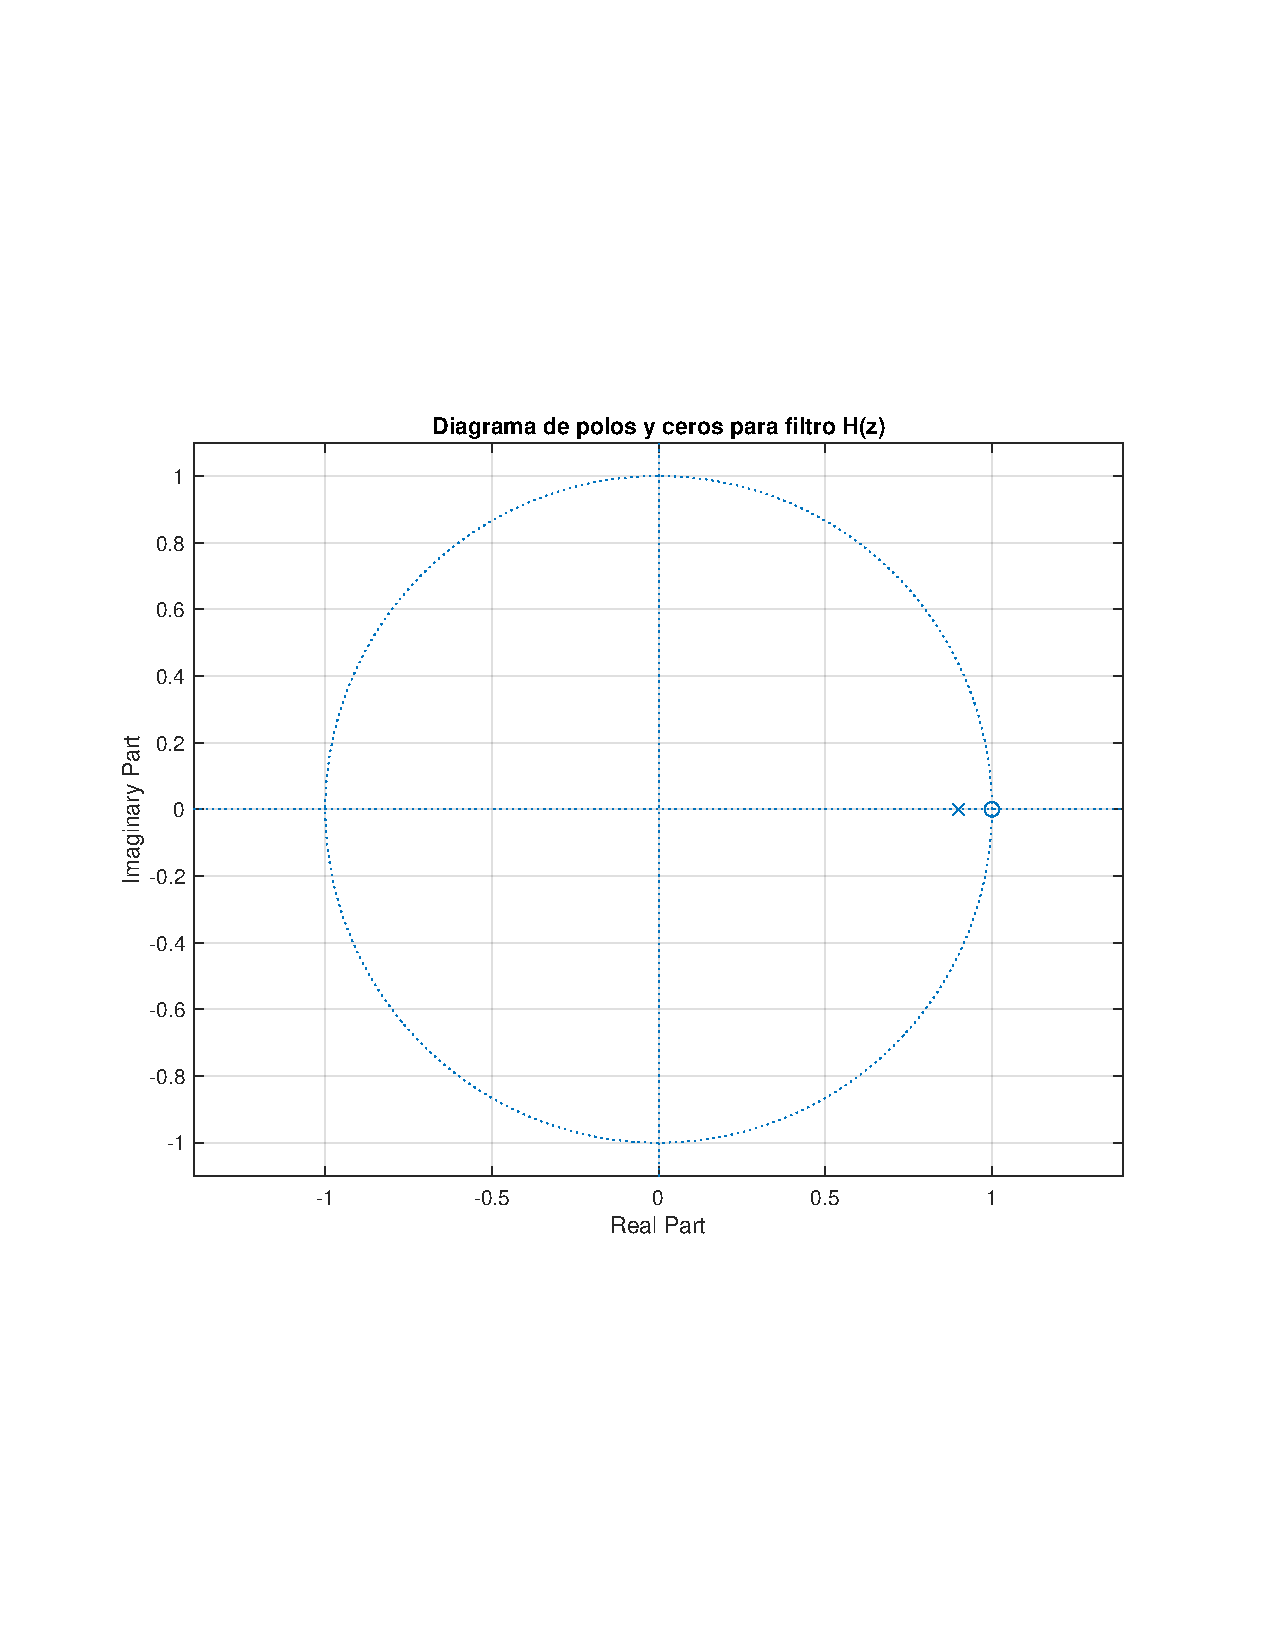
\includegraphics[width=0.6\textwidth,clip, trim = {1.9cm 6.8cm 2.3cm 7cm}]{../plots/1_zp_diag.pdf}
			\caption{Diagrama de polos y ceros para la función de transferencia \ref{eq:1_filter_transfer_function}}
			\label{fig:1_zero_pole_diagram}
		\end{figure}
		
		Analizando la respuesta en magnitud y fase del filtro:
		\begin{figure}[H]
			\center
			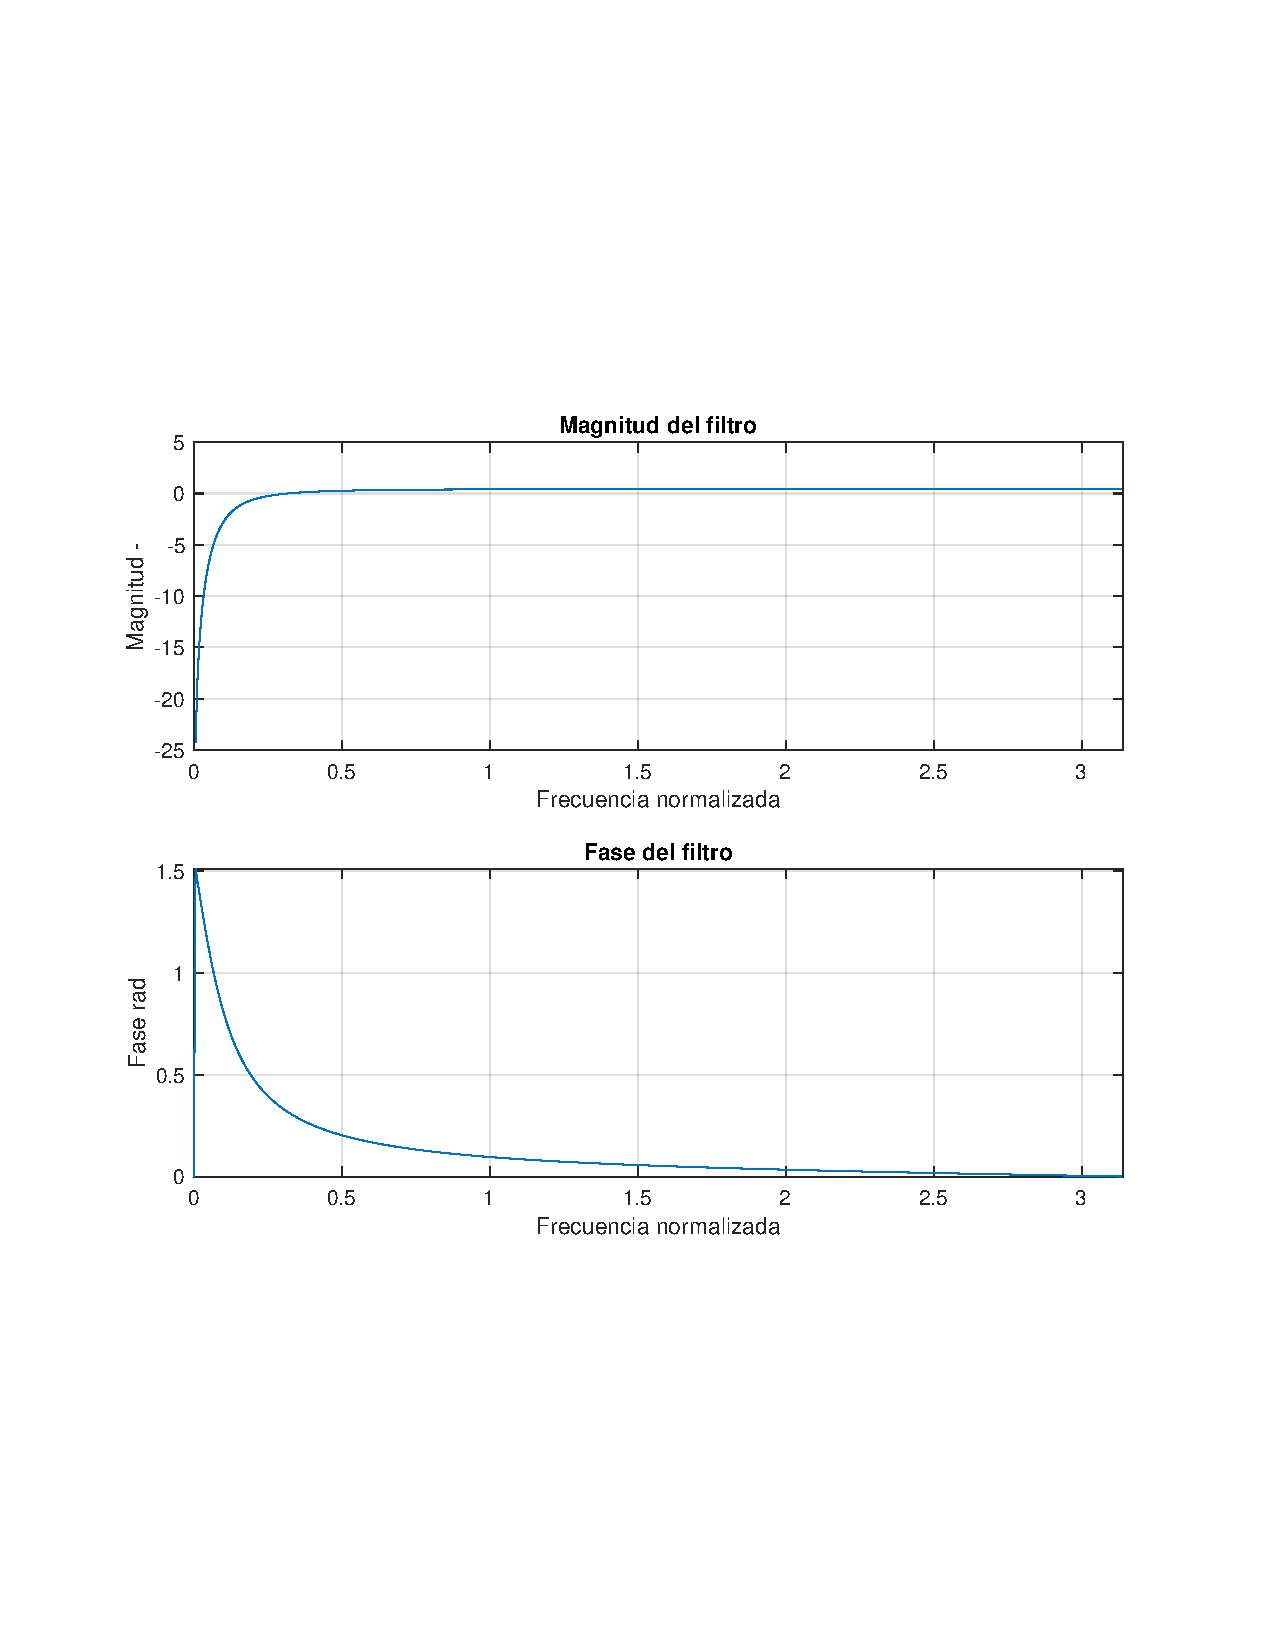
\includegraphics[width=0.6\textwidth,clip, trim = {1.9cm 6.8cm 2.3cm 7cm}]{../plots/1_mag_phase.pdf}
			\caption{Respuesta en magnitud y fase para el filtro}
		\end{figure}
		
		Se procede a evaluar la función \ref{eq:1_filter_transfer_function}, para $\omega = pi$:
		
		\begin{equation}
			H(\pi) = \frac{e^{j\pi} - 1}{e^{j\pi} - 0.9} = \frac{-2}{-1,9} \approx 1.0526
			\label{eq:1_filter_pi}
		\end{equation}
		
		Para normalizar la respuesta del filtro, para $\omega = \pi$, basta con hacer que para esta frecuencia el filtro tenga ganancia unitaria, por lo que se puede definir la ganancia de normalización:
		\begin{equation}
			G_{n} = \frac{1.9}{2} = 0.95
		\end{equation}
		
		Por lo que se puede reescribir la función de transferencia:
		\begin{equation}
			\hat{H}(z) = G_{n} \cdot H(z) = 0.95 \cdot \frac{z - 1}{z -0.9} 
			\label{eq:1_transfer_function_normal}
		\end{equation}
		
		Llevando la expresión a su forma de ecuación de diferencias:
		\begin{align}
			X(z) \cdot 0.95 ( 1 - z^{-1} ) = Y(z) \cdot (1 - 0.9 z^{-1}) \\
			y(z) = 0.9 \cdot y\left[ n - 1 \right] + 0.95 \left( x\left[ n - 1 \right] - x\left[n \right] \right)
		\end{align}
		
		\textcolor{red}{TERMINAR DEMOSTRACIONES - VERIFICAR}
		
		 Considere ahora, que se tiene como entrada del filtro definido en \ref{eq:1_transfer_function_normal}:
		 \begin{equation*}
		 	x[n] = 2 \cdot cos \left( \frac{\pi}{6}n + \frac{\pi}{4} \right)
		 \end{equation*}
		 
		Como se sabe, la expresión tiene una única frecuencia fundamental en $\pm \pi/6$. De esta forma, para el filtro diseñado en el punto anterior, basta evaluar únicamente el efecto de la atenuación y desfase para la frecuencia de la señal de entrada. De esta forma:
		\begin{align}
			|H(\pi/6)| = 0.95 \cdot \left| \frac{e^{j\pi/6} - 1}{e^{j\pi/6} - 0.9} \right| = 0.9812 \\
			\angle H(\pi/6) = arctan\left( 0.95 \cdot \frac{e^{j\pi/6} - 1}{e^{j\pi/6} - 0.9} \right) = 0.1940~\text{rad} 
		\end{align}
		
		De esta forma, se puede obtener la salida:
		\begin{equation}
			y[n] = \sqrt(2) \cdot 0.9812 \cdot cos \left( \frac{\pi n}{6} + \frac{\pi}{4} + 0.1940 \right)
		\end{equation}
		
	\subsection{Filtraje señal electrocardiograma}
		Se pide diseñar un filtro con dos ceros, para el filtraje de una señal ECG muestreada a 200~Hz, con ruido en la banda de 60~Hz. Analizando la señal:
		\begin{figure}[H]
			\center
			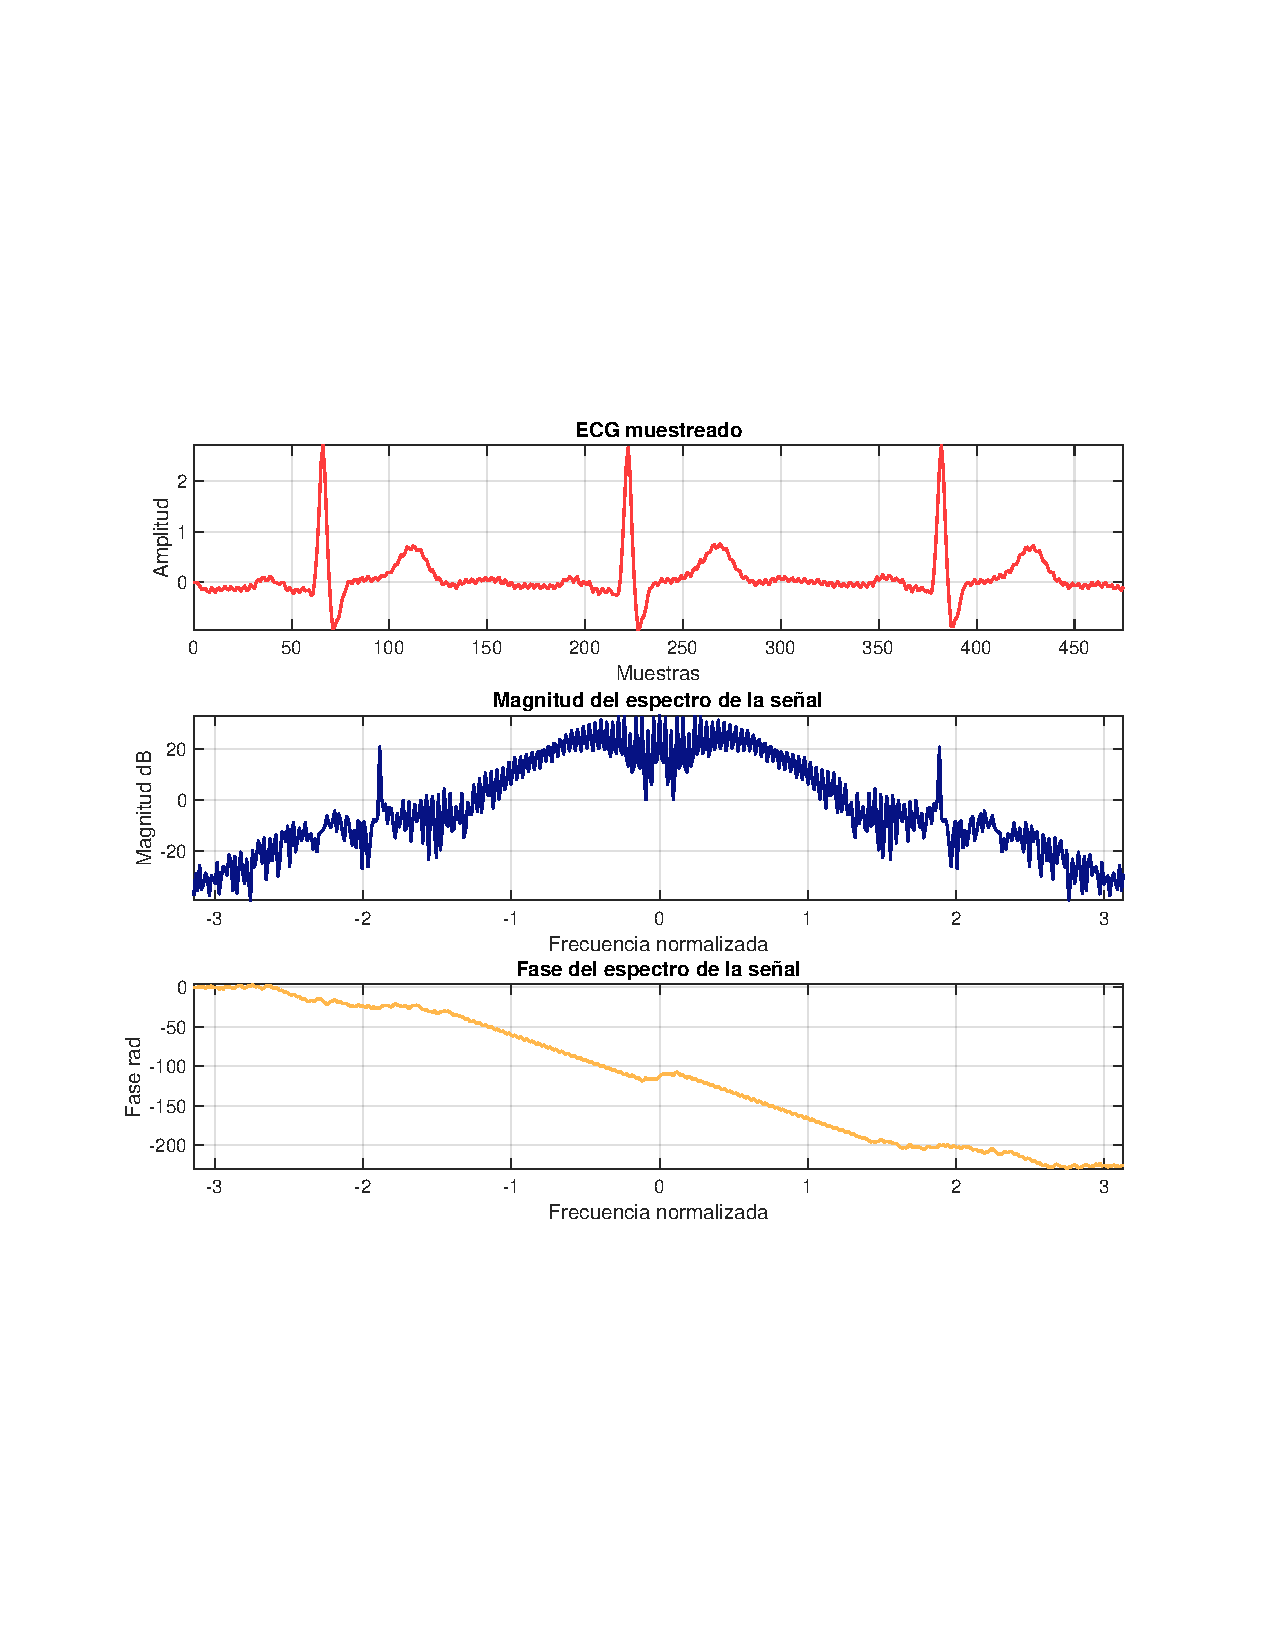
\includegraphics[width=0.6\textwidth,clip, trim = {1.9cm 6.8cm 2.3cm 7cm}]{../plots/ecg_time_freq.pdf}
			\caption{Señal muestreada, en el dominio temporal y de frecuencia}
			\label{fig:ecg_time_freq}
		\end{figure}		
				
		Se puede ver claramente, las bandas de ruido presentes. Se propone la siguiente estructura para el filtro:
		\begin{align}
			\omega_{r} = \frac{2\pi 60}{200} = 0.6\pi \\
			H(z) = \frac{(z-e^{j\omega_r})(z-e^{-j\omega_r})}{z^{2}} = \frac{z^{2} + 2cos(\omega_{r}) + 1}{z^{2}}
		\end{align}
		
		Realizando la implementación en \textsc{Matlab}, se puede obtener la magnitud y fase del filtro:
		\begin{figure}[H]
			\center
			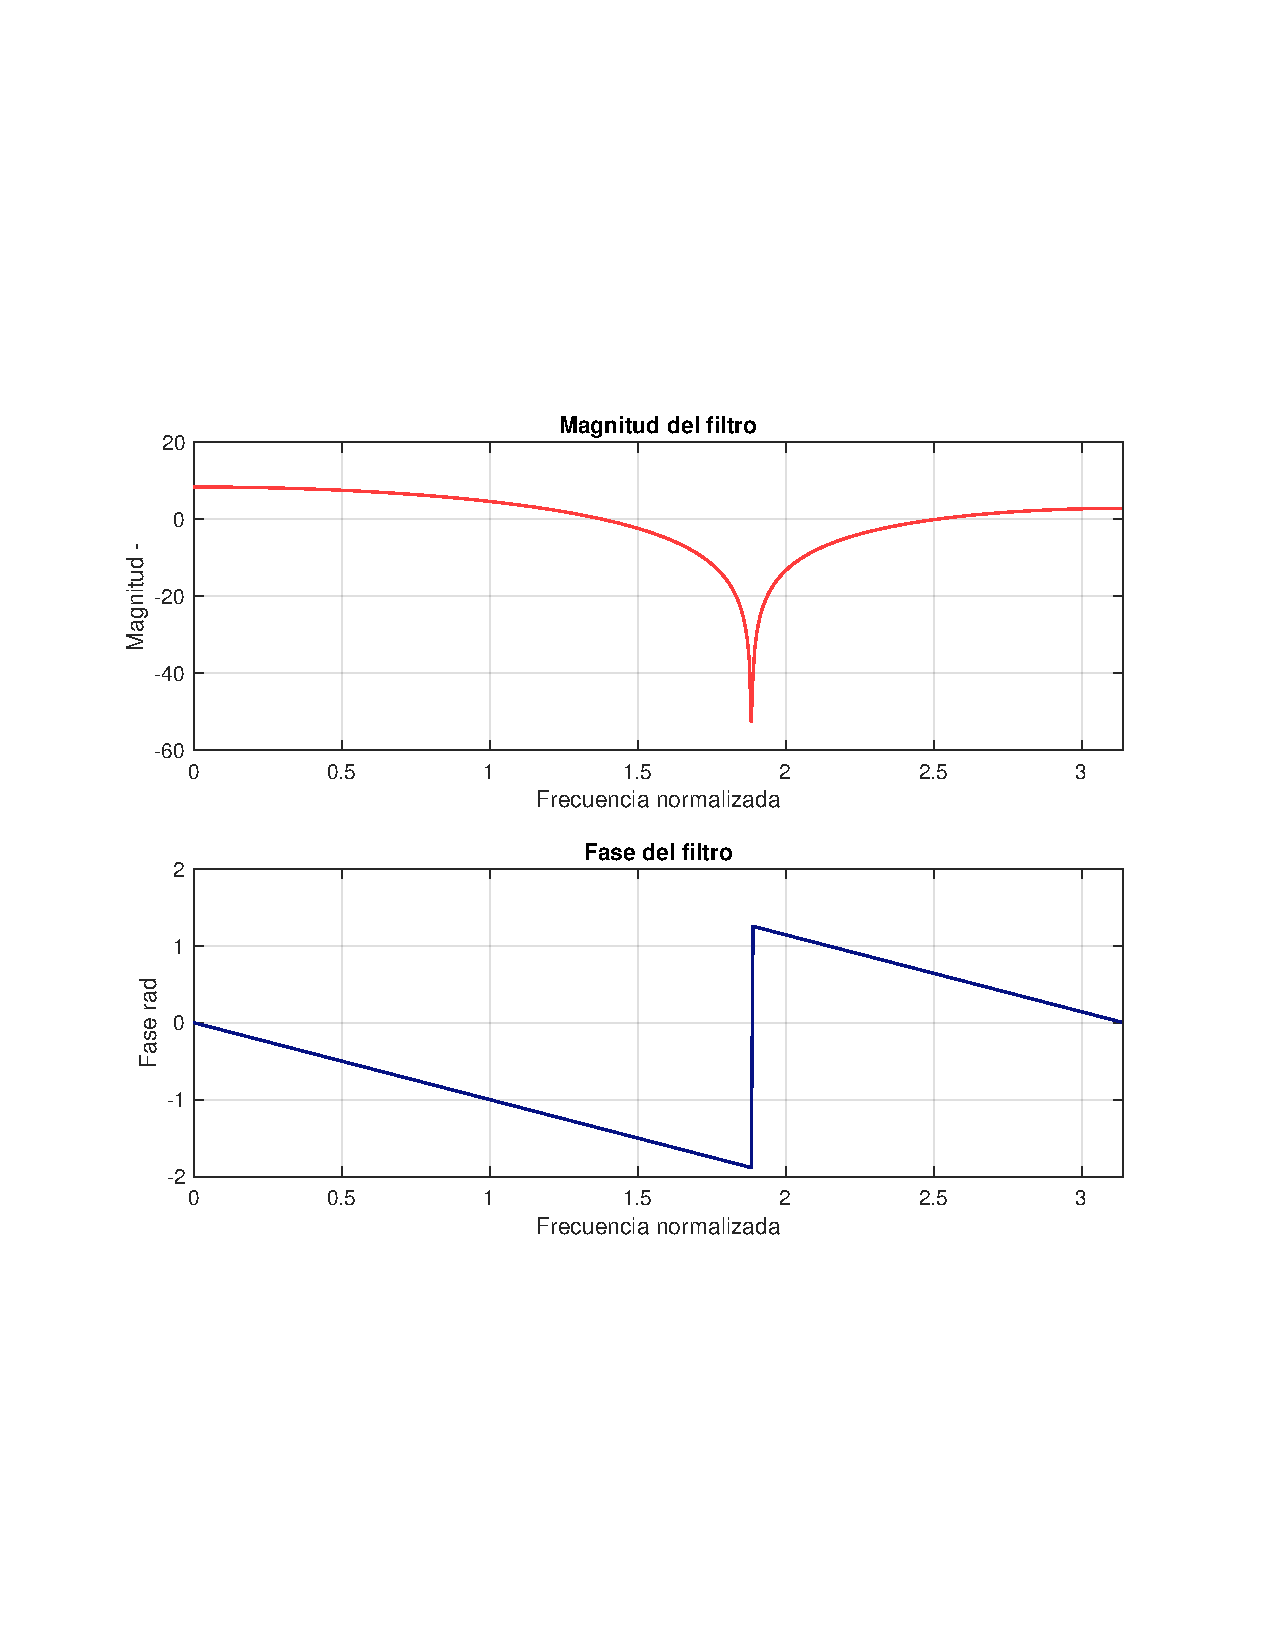
\includegraphics[width=0.6\textwidth,clip, trim = {1.9cm 6.8cm 2.3cm 7cm}]{../plots/ecg_poles_0.pdf}
			\caption{Respuesta en magnitud y fase para el filtro}
			\label{fig:mag_phase_p_0}
		\end{figure}
		
		A partir de las respuestas del filtro, se puede ver que en términos de magnitud, tiene un rechazo relativamente lento, con la banda de paso no plana. En términos de la fase, se puede ver que se tiene un desfase lineal deseable. Aplicando el filtro a la señal:
		
		\begin{figure}[H]
			\center
			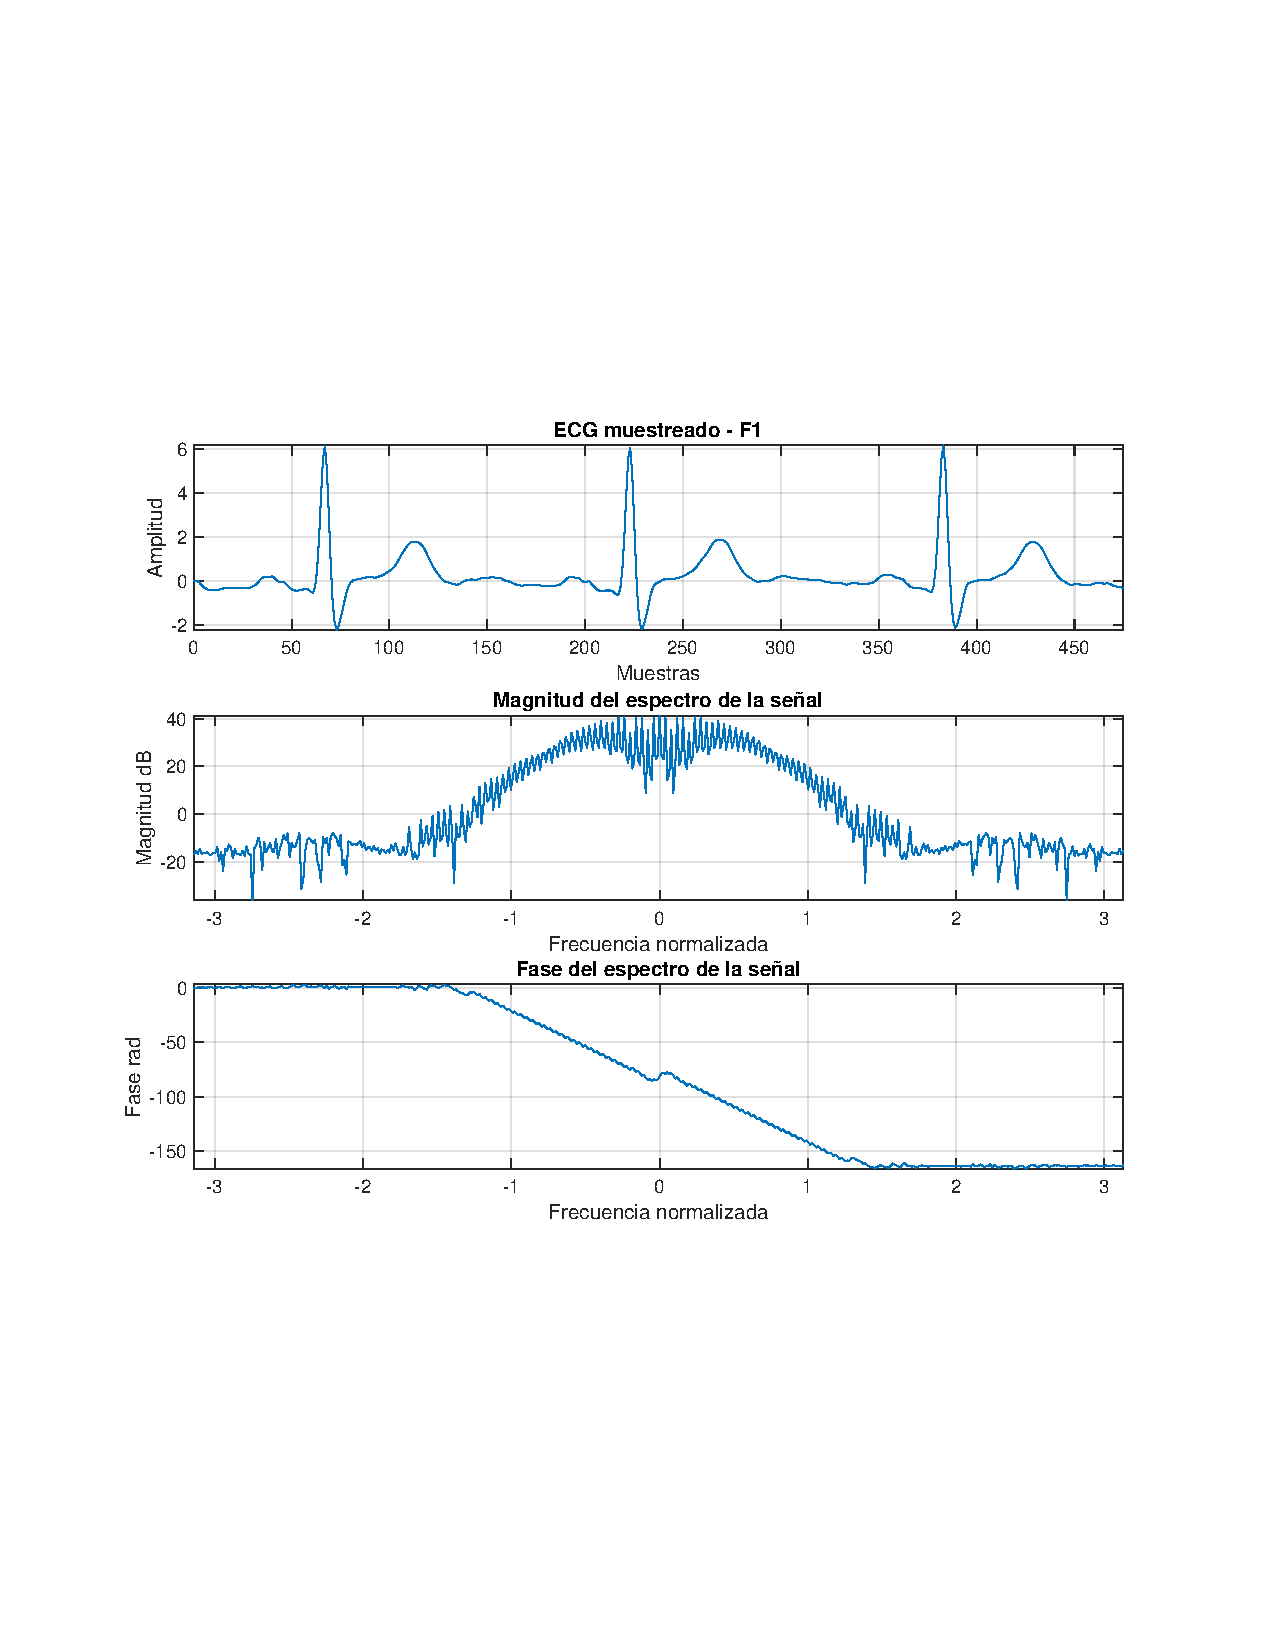
\includegraphics[width=0.6\textwidth,clip, trim = {1.9cm 6.8cm 2.3cm 7cm}]{../plots/ecg_poles_0_filtered.pdf}
			\caption{Resultado del filtraje de la señal}
			\label{fig:ecg_filtered_0}
		\end{figure}
		
		Se puede ver que el proceso de filtrado ha sido exitoso, permitiendo remover la banda con ruido de la señal. Se puede ver una cierta \textit{amplificación} de ciertas bandas, dada la forma no plana del filtro, el espectro se tendió a \textit{curvar}. En términos de fase, se puede ver que el efecto del filtro sobre ésta, es el esperado, dada la fase lineal del filtro. Realizando una comparación directa de ambas señales:
		\begin{figure}[H]
			\center
			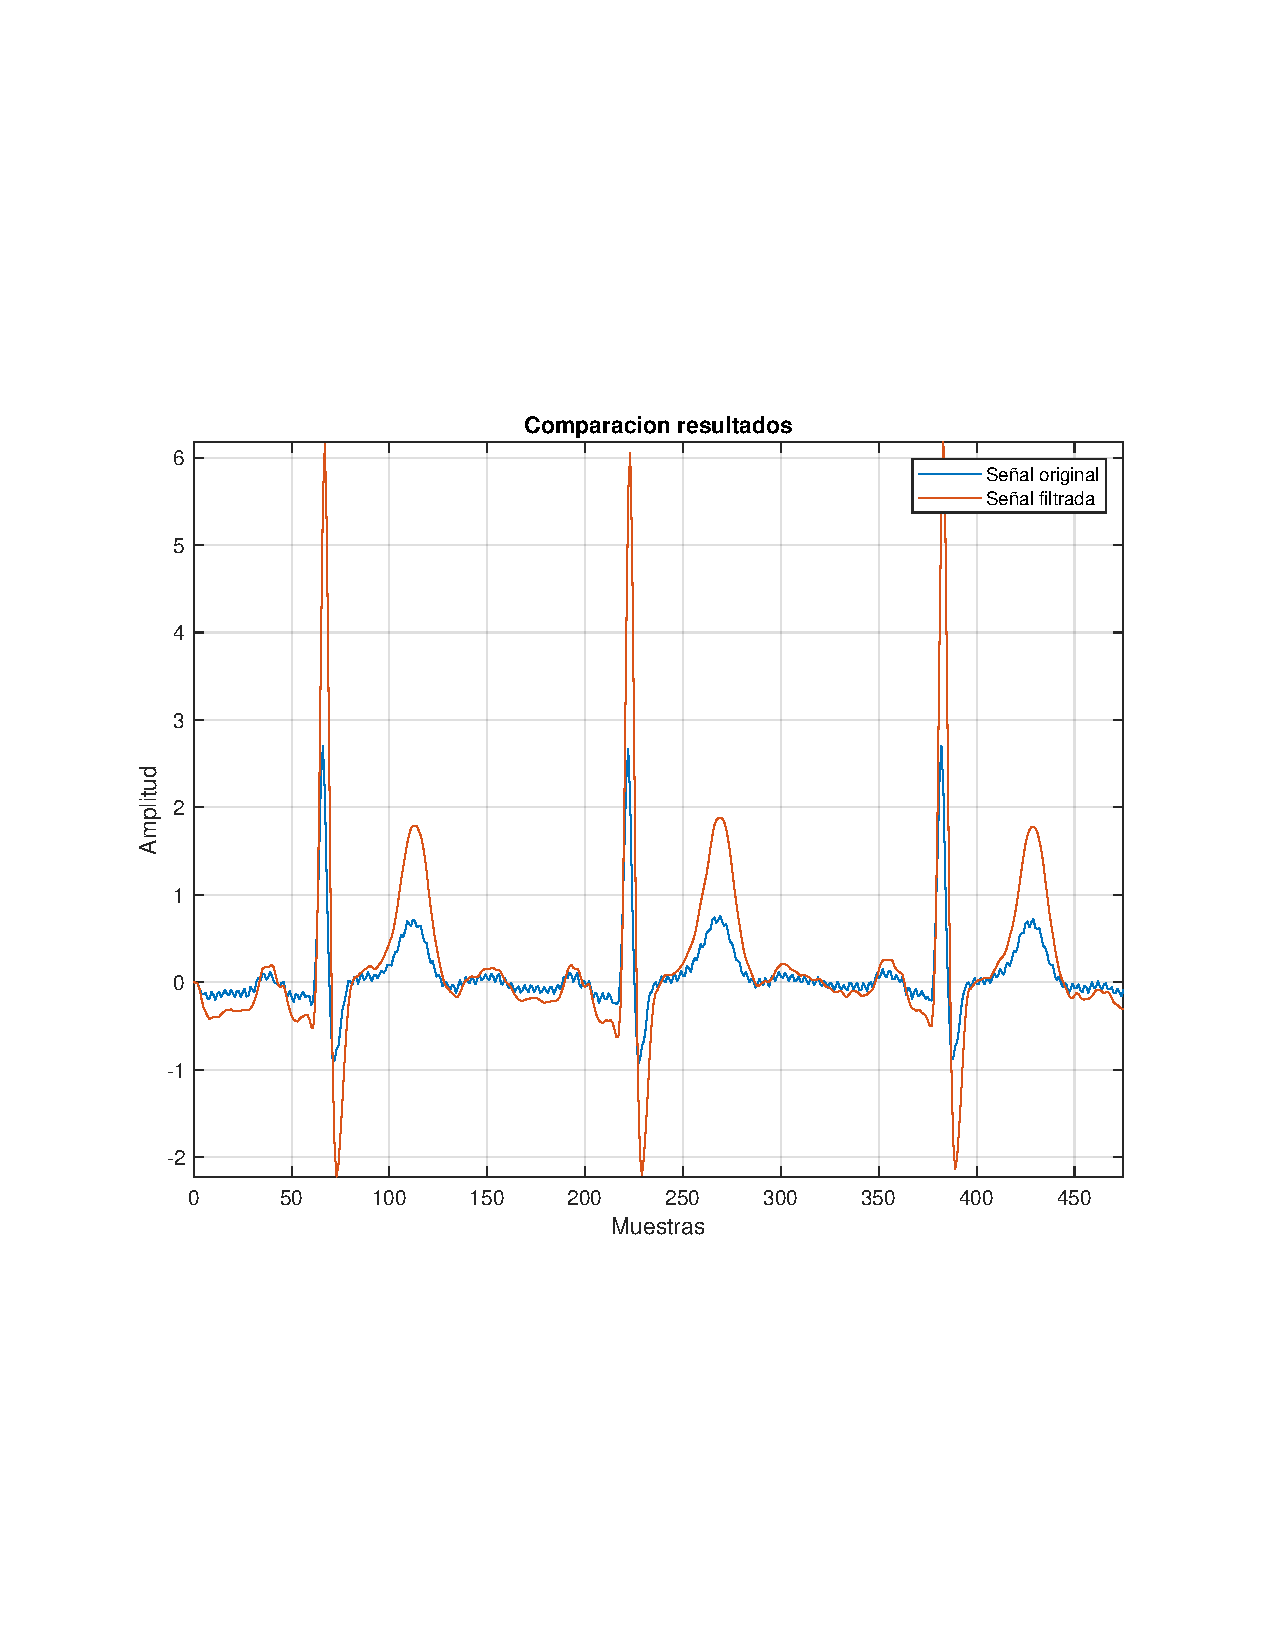
\includegraphics[width=0.6\textwidth,clip, trim = {1.9cm 6.8cm 2.3cm 7cm}]{../plots/egc_f_0_comparative.pdf}
			\caption{Comparación de las señales}
			\label{fig:ecg_filtered_0_comparative}
		\end{figure}
		
		Considere ahora, que se añaden dos polos a la frecuencia de rechazo, con un radio $r \in [0,8  - 0,99]$. A partir de esto, se escogen tres valores para $r = 0.8, r = 0.9, r = 0.99$. Implementando los filtros y comparando su respuesta en magnitud y frecuencia:
		\begin{figure}[H]
			\center
			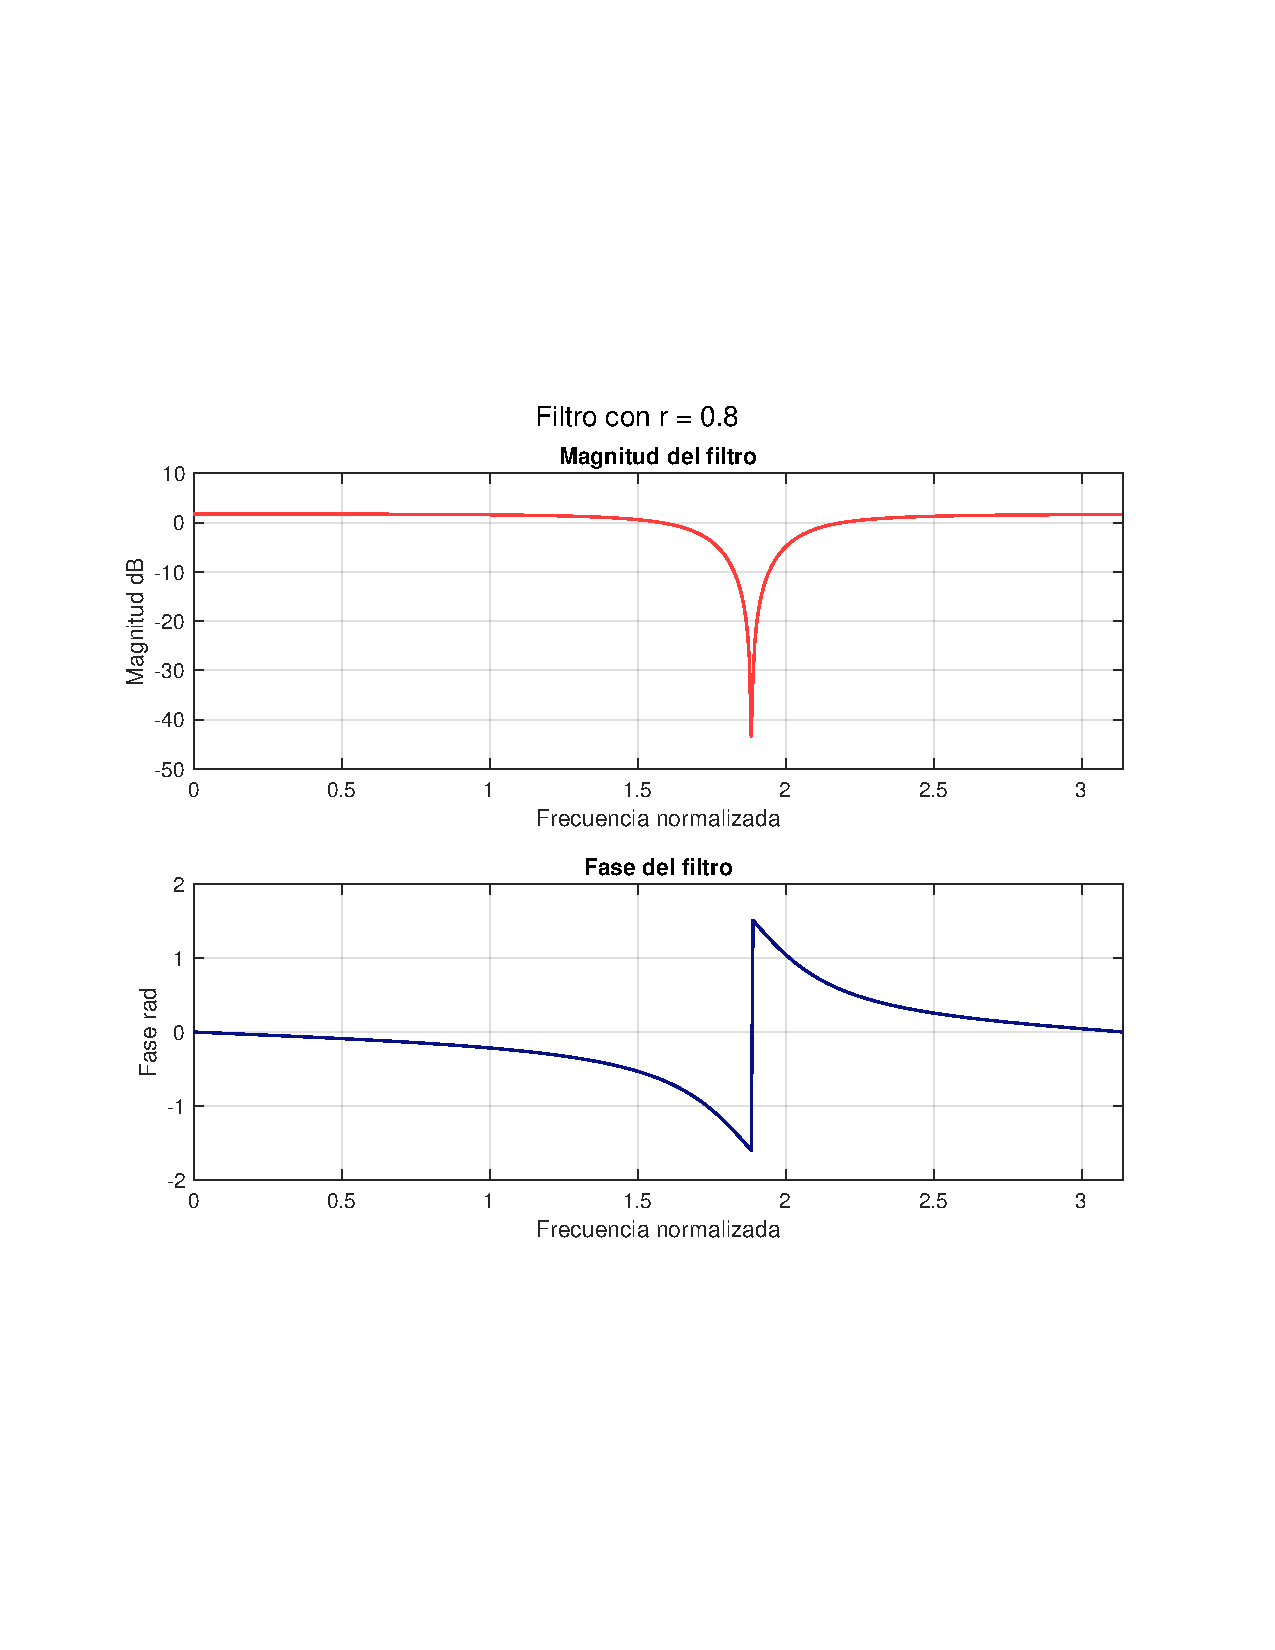
\includegraphics[width=0.6\textwidth,clip, trim = {1.9cm 6.8cm 2.3cm 7cm}]{../plots/ecg_poles_208.pdf}
			\caption{Respuesta del filtro, para r = 0.8}
			\label{fig:ecg_filter_r_08}
		\end{figure}

		\begin{figure}[H]
			\center
			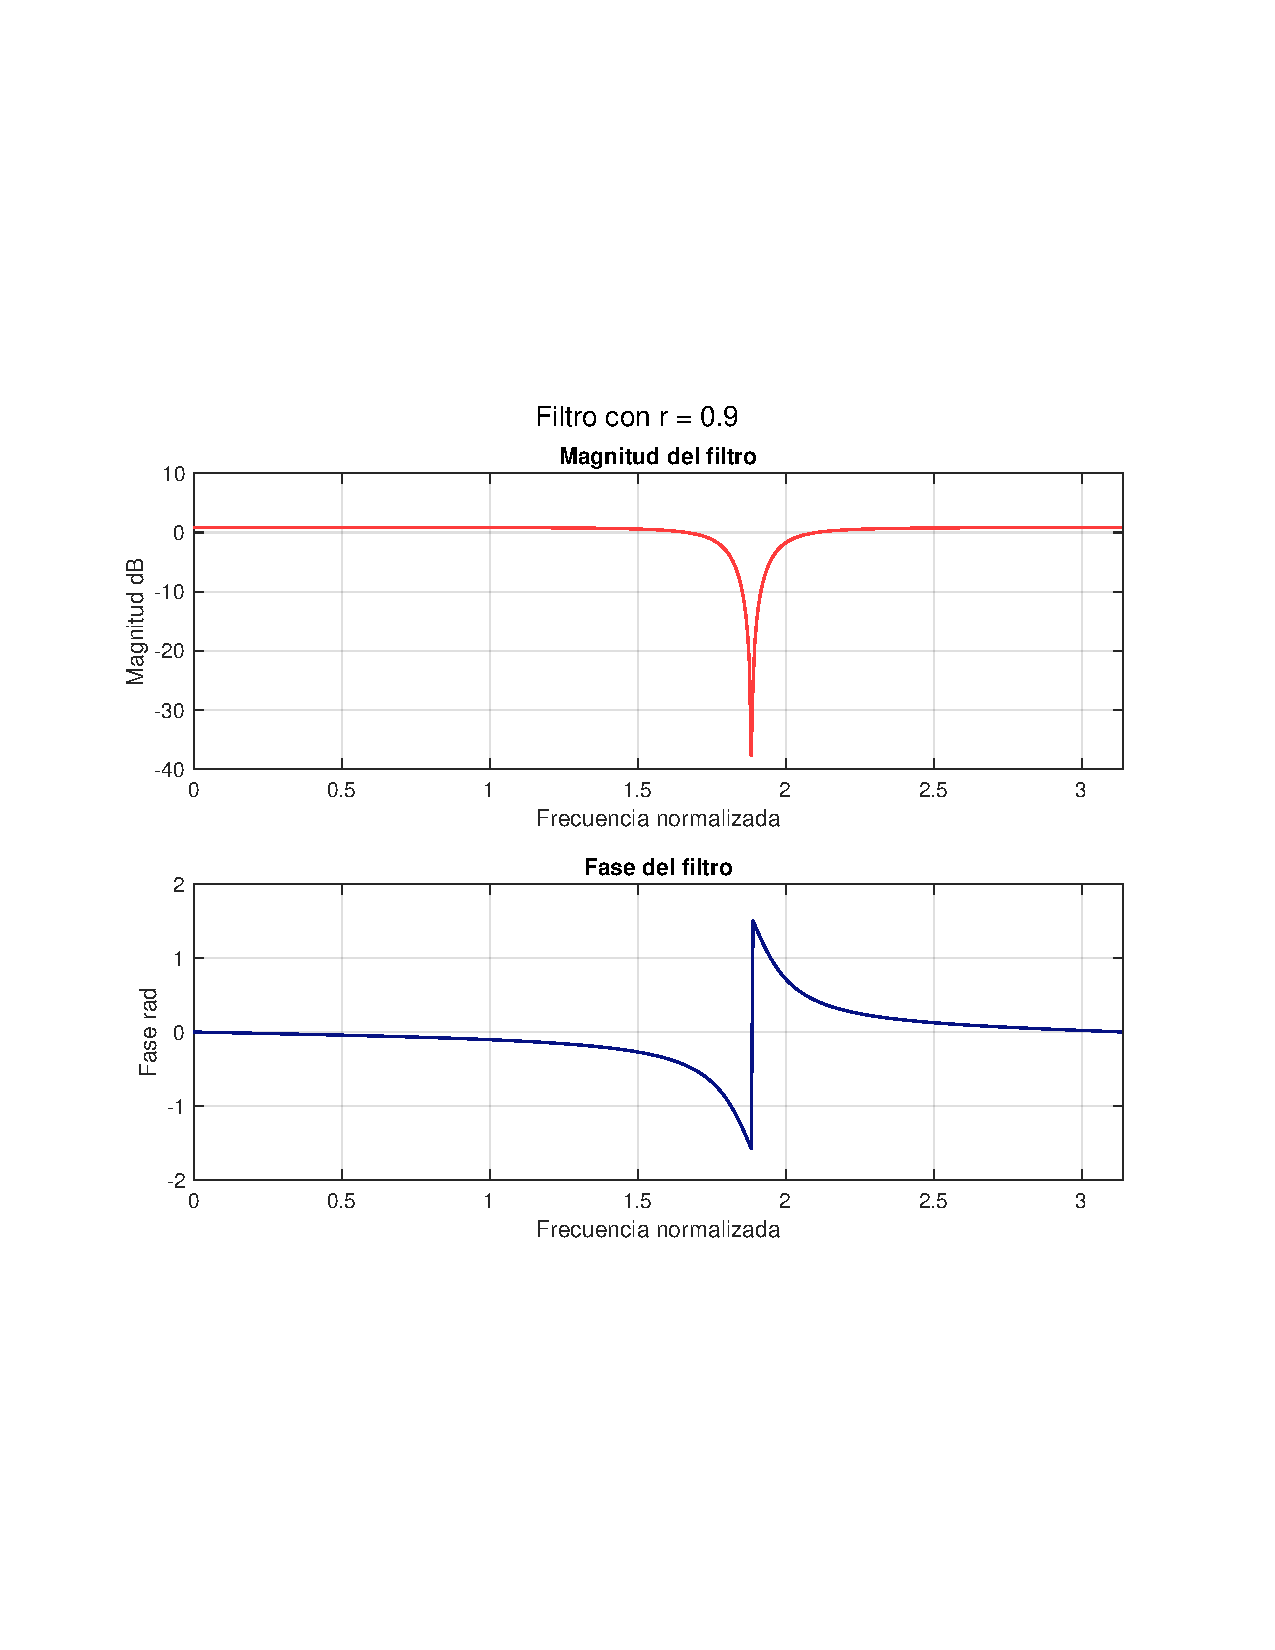
\includegraphics[width=0.6\textwidth,clip, trim = {1.9cm 6.8cm 2.3cm 7cm}]{../plots/ecg_poles_209.pdf}
			\caption{Respuesta del filtro, para r = 0.9}
			\label{fig:ecg_filter_r_09}
		\end{figure}		
		
		\begin{figure}[H]
			\center
			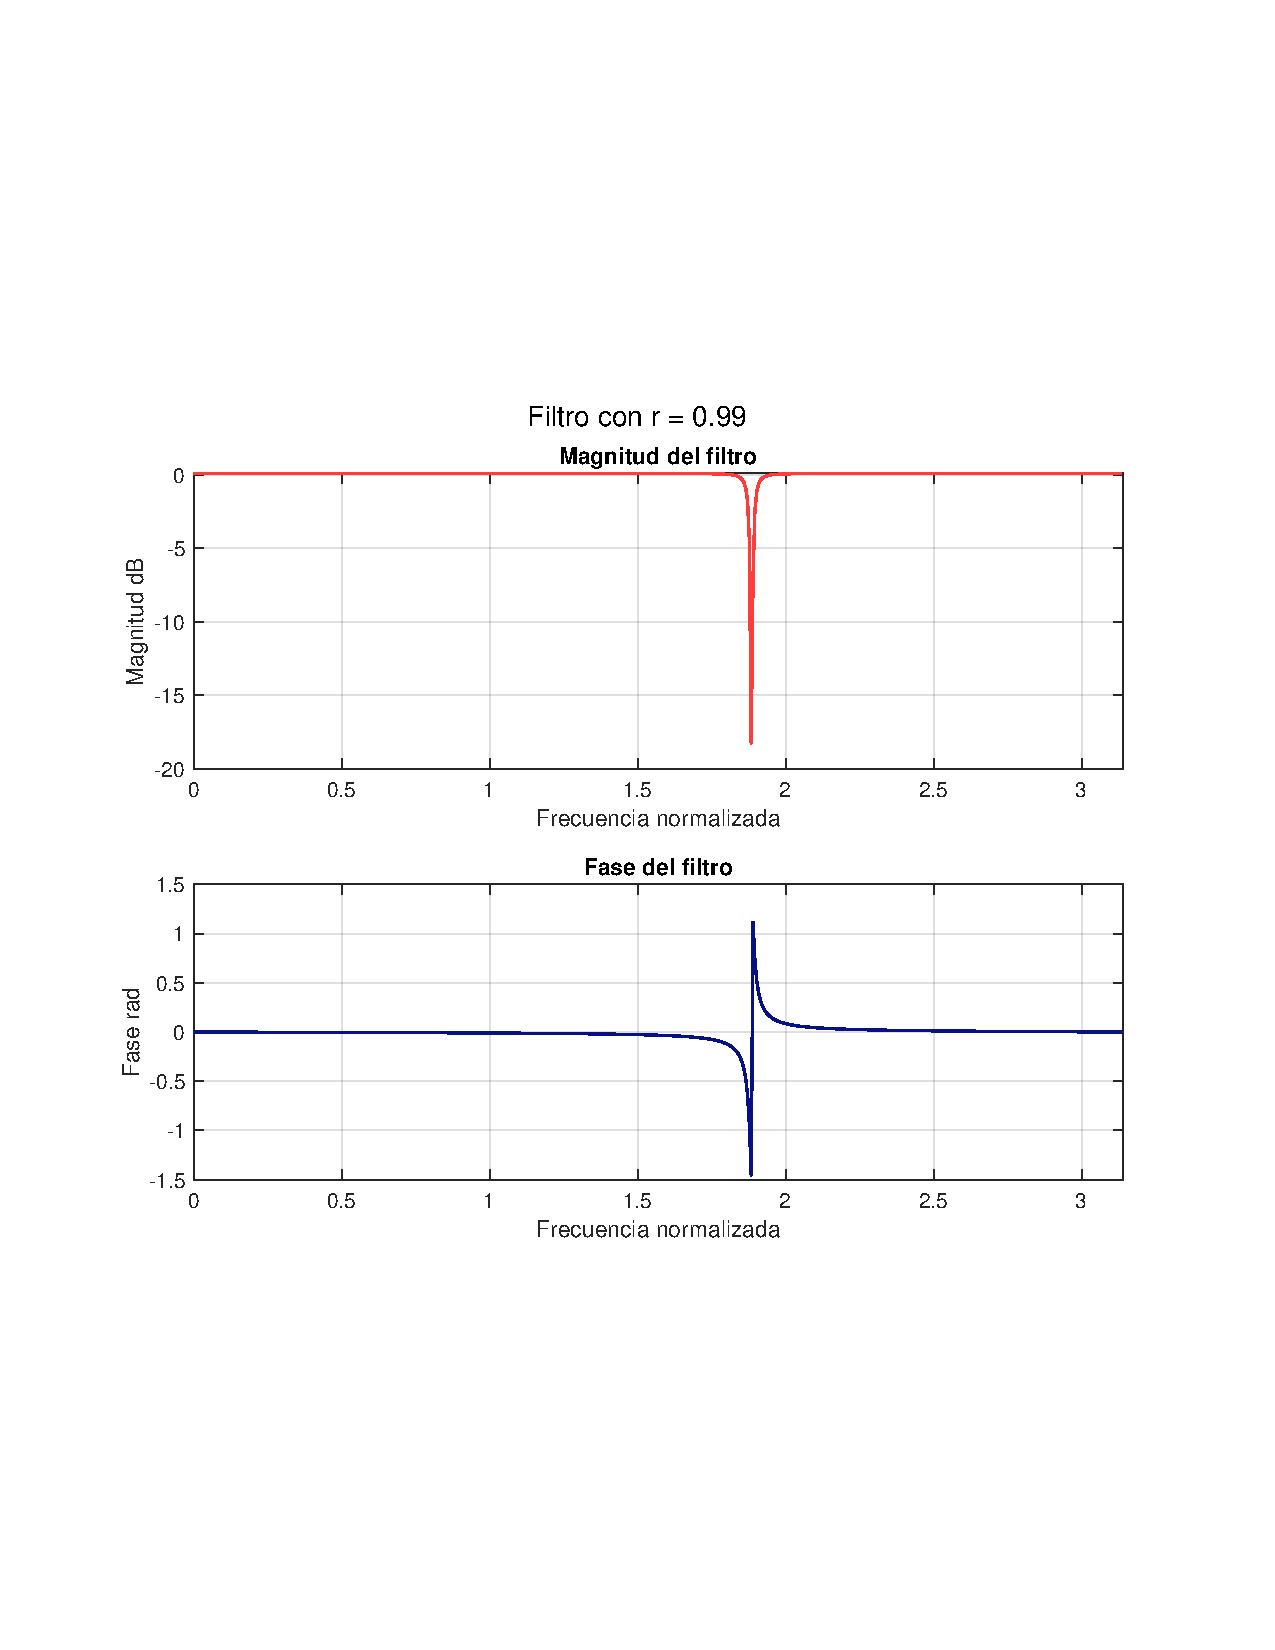
\includegraphics[width=0.6\textwidth,clip, trim = {1.9cm 6.8cm 2.3cm 7cm}]{../plots/ecg_poles_2099.pdf}
			\caption{Respuesta del filtro, para r = 0.99}
			\label{fig:ecg_filter_r_099}
		\end{figure}
		
		A partir de estos resultados, se puede comprobar que a medida que el valor de $r$, se acerca al círculo unitario, la banda de rechazo se hace mas angosta, acercándose lo más posible a la respuesta ideal de un filtro \textit{notch}, sin embargo, esta mejora en el rechazo del filtro, trae consigo que la fase, que inicialmente era ``perfectamente'' lineal, se empieza a curvar en torno a la banda de rechazo. Por lo tanto al construir el filtro, se debe tener en cuenta la aplicación final, dado que determinará si es factible tener un mejor rechazo a costa de una fase no lineal. La mejora en el rechazo del filtro, se puede explicar, si consideramos que un cero anula la función de transferencia, mientras que un polo la \textit{indefine}, por lo que entre mas cerca esté el polo del cero, la recuperación de la anulación en el espectro será mejor y más rápida, dando un filtro más selectivo. Otro punto a destacar, es que a medida que el valor de r se acerca al círculo unitario, la respuesta en magnitud se hace más plana, eliminando la curvatura del espectro que se tenía para el filtro con polos en cero, figura \ref{fig:mag_phase_p_0}. Tomando el caso para $r = 0.99$, se filtra la señal ECG entregada, obteniéndose el siguiente resultado:
		
		\begin{figure}[H]
			\center
			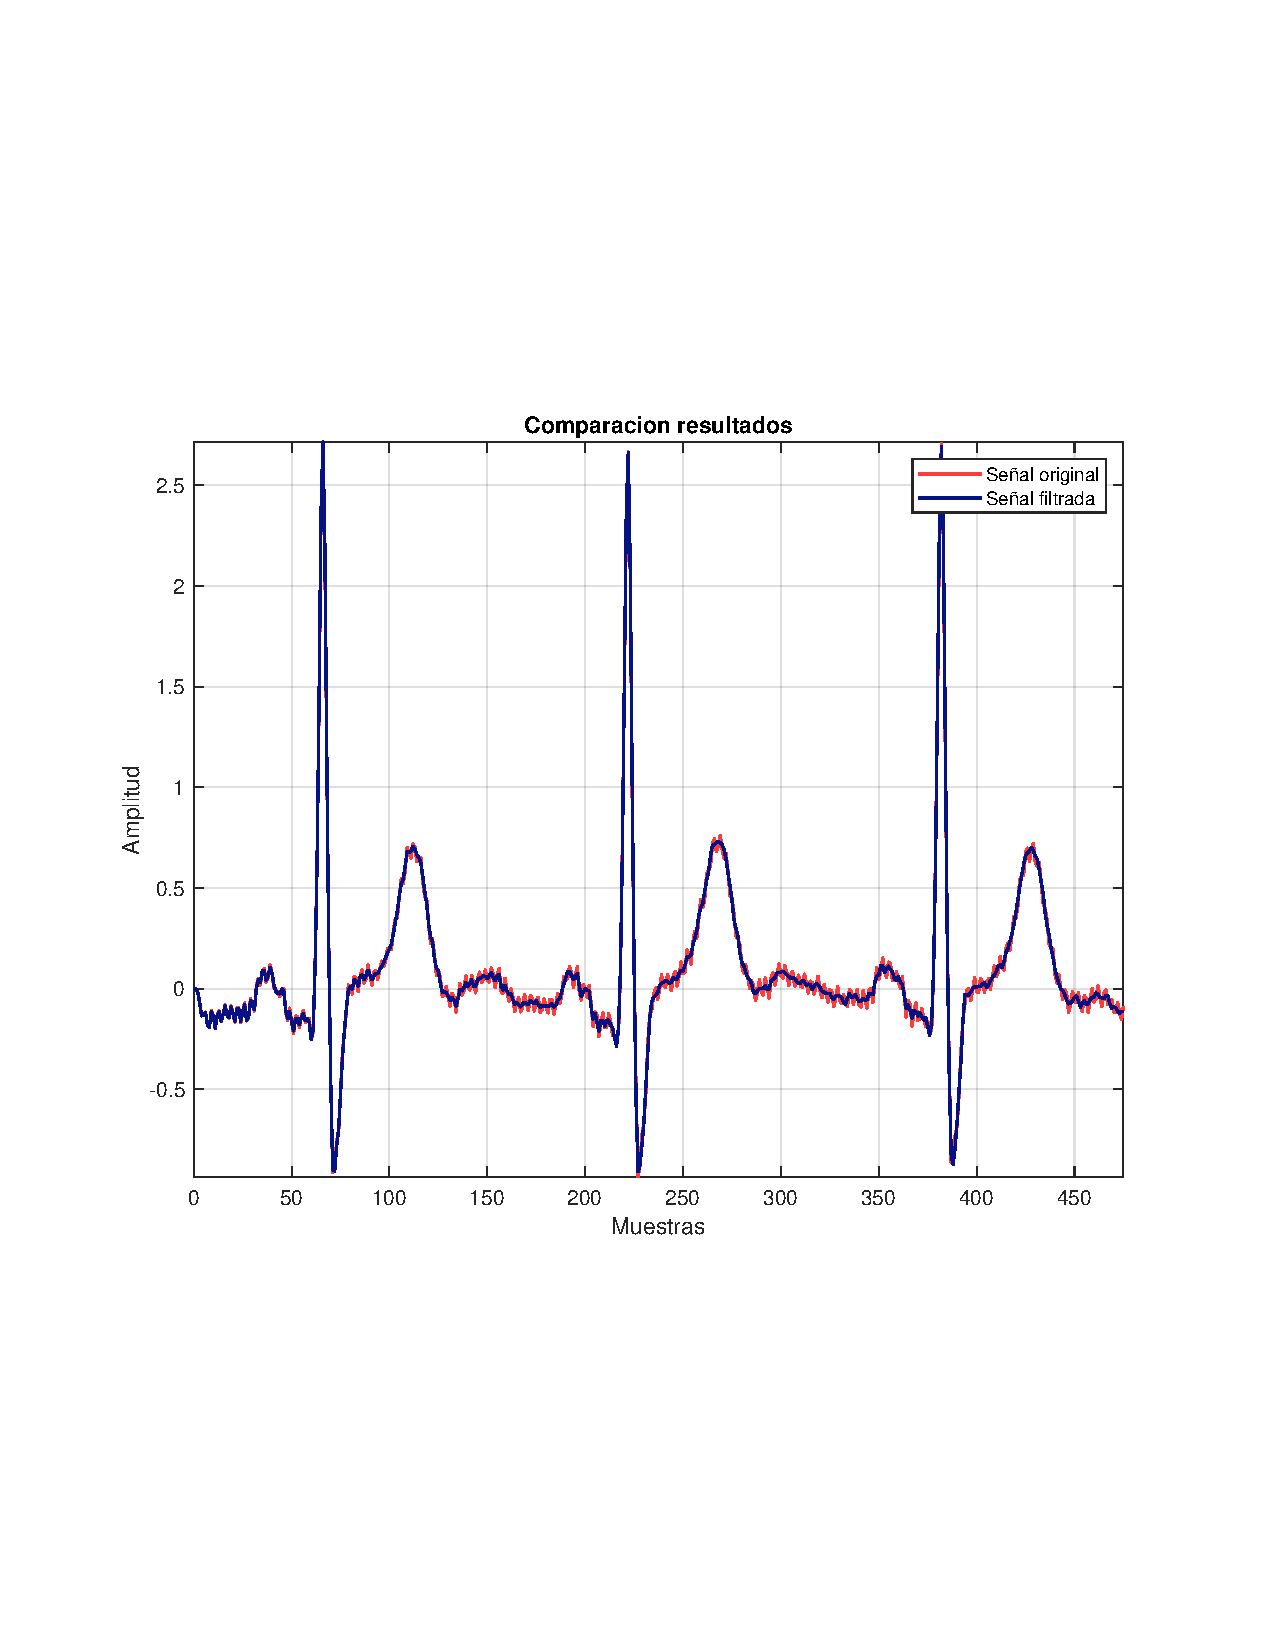
\includegraphics[width=0.6\textwidth,clip, trim = {1.9cm 6.8cm 2.3cm 7cm}]{../plots/egc_f_2_comparative.pdf}
			\caption{Resultado de filtraje, para r = 0.99}
			\label{fig:ecg_filter_r_099_result}
		\end{figure}
		
		A partir de esto, se puede comprobar, que se tiene un mejor filtrado de la señal, y que el efecto causado por la fase no lineal, no es apreciable. La respuesta más plana en frecuencia, permite que el filtro siga de manera más cercana la señal original, sin tener efectos de amplificación, como en el caso de polos en cero. Por lo que para esta aplicación el filtro diseñado para $r = 0.99$ es una buena solución. 
		
		
	
	